\documentclass[11pt]{paper}
\usepackage[frenchb]{babel}

\usepackage[T1]{fontenc}

\usepackage{graphicx}
\usepackage{amssymb}
\usepackage{amstext}
\usepackage{amsmath}
\usepackage{a4wide,color}
\usepackage[utf8]{inputenc}
\usepackage{xspace}
\usepackage{anysize}
\usepackage{tabularx}
\usepackage{multirow}
\usepackage{fancybox}
\usepackage{fancyhdr}
\usepackage{bbding}

\setlength{\parskip}{1ex plus 0.5ex minus 0.2ex}

\usepackage{threeparttable}
\usepackage{color}
\usepackage{float}

\usepackage[toc,page]{appendix} 
\usepackage{lscape}
\usepackage{xspace}

\usepackage{placeins}

\usepackage{listingsutf8}

\usepackage{todonotes}

\lstset{% general command to set parameter(s)
	basicstyle=\footnotesize, % print whole listing small
	keywordstyle=\color{magenta}\bfseries, % underlined bold black keywords
	identifierstyle=, % nothing happens
	commentstyle=\color{black}, % white comments
	stringstyle=\ttfamily, % typewriter type for strings
	showstringspaces=false % no special string spaces
} 

\lstdefinelanguage{aald}
	{morekeywords={system, implementation},
	sensitive=false,
	morecomment=[l]{//},
	morecomment=[s]{/*}{*/},
	morestring=[b]",
}

\usepackage[colorlinks=true]{hyperref}

\usepackage[normalem]{ulem}
\usepackage{color}

\definecolor{Fond}{gray}{0.9}

\renewcommand{\floatpagefraction}{.99}
\renewcommand{\textfraction}{.01}
\newcommand{\modif}[1]{\textcolor{red}{\uline{#1}}}

\newcounter{cptreq}
\newcommand{\req}[1]{
\stepcounter{cptreq}
	\noindent\fcolorbox{black}{Fond}{%                couleur du texte, couleur du fond
		\begin{minipage}[t]{\textwidth}
		{\bf Fonctionnalité \thecptreq}\, :  #1
		\end{minipage}
	}
}

\newcommand{\raspi}{Raspberry Pi\xspace}

\pagestyle{fancy}
\fancyhf{}
\fancyhead[RE,RO]{\thepage}
\fancyhead[LE]{}
\fancyhead[LO]{Programmation et conception de systémes temps réel -- 4éme année AE/IR}
\fancyfoot[LO]{INSA Toulouse — P.-E. Hladik}
\fancypagestyle{plain}{%
  \fancyhf{} % get rid of headers
  \renewcommand{\headrulewidth}{0pt} % and the line
}

\newenvironment{maliste}%
{ \begin{list}%
	{\ArrowBoldRightStrobe}%
	{\setlength{\labelwidth}{30pt}%
	 \setlength{\leftmargin}{35pt}%
	 \setlength{\itemsep}{\parsep}}}%
{ \end{list} }

\renewcommand{\appendixtocname}{Annexes} 
\renewcommand{\appendixpagename}{Annexes}


\title{{\Huge Projet De Stijl 2.0}
{\small : Plateforme pour robots mobiles}\\
{\scriptsize Programmation et conception de systémes temps réel -- 4éme année AE/IR}\\
{\scriptsize Institut National des Sciences Appliquées de Toulouse}\\
---\\
Guide des outils de développement \\
{\large Version 1.0.$\beta$ (\today)}\\
{\scriptsize Référent pédagogique : P.-E. Hladik (\texttt{pehladik@insa-toulouse.fr})}\\
{\scriptsize Référents plateforme : S. Di Mercurio (\texttt{dimercur@insa-toulouse.fr})}\\
---
}



\begin{document}


\maketitle

%%%%%%%%%%%%%%%%%%%%
\section{Code initial du projet}
\label{sec:git}
%%%%%%%%%%%%%%%%%%%%

Le code du projet est disponible sur un dépôt git hébergé sur GitHub. Pour le récupérer, placer vous le répertoire cible et exécuter la commande\\ \indent\indent {\tt git clone https://github.com/INSA-GEI/dumber.git}

Il vous faut ensuite changer de branche, pour cela allez dans le répertoire {\tt dumber} puis exécuter la commande\\ \indent\indent {\tt git checkout stable}
 
Tout le code relatif au projet est disponible, cependant vous n'aurez besoin que des codes présents dans les répertoires :
\begin{itemize}
	\item {\tt ./dumber/software/raspberry}
	\item {\tt ./dumber/software/monitor/monitor}
\end{itemize}

 \todo[inline]{Mettre à jour la suite en fonction du projet initial}
  
 Vous aurez alors un répertoire {\tt ./dumber/software} dans lequel vous trouverez les répertoires:
 \begin{itemize}
\item {\tt /src} avec le codes des librairies du projet,
\item {\tt /destijl\_init} avec le codes correspondant au projet initial,
\item {\tt /example} avec des codes d'exemple pour utiliser les librairies (attention ce n'est pas à jour).\\
\end{itemize}


Le code du projet initial est constitué des fichiers suivants :
\begin{itemize}
\item {\tt /destijl\_init/main.cpp} qui contient le main de l'application et les fonctions de création des objets (tâches, sémaphores, mutex, etc.) de l'architecture logicielle,
\item {\tt /destijl\_init/src/functions.cpp} qui contient l'implémentation des fonctions,
\item {\tt /destijl\_init/src/functions.h} qui contient l'entête des différentes fonctions.\\
\end{itemize}

A cela s'ajoute un fichier {\tt Makefile} disponible dans {\tt /destijl\_init} qui permet de compiler le projet initial sur une \raspi.


%%%%%%%%%%%%%%%%%%%%
\section{Mise en place d'un terminal distant sur la \raspi}
\label{sec:ssh}
%%%%%%%%%%%%%%%%%%%%

Pour se connecter à la \raspi, vous aurez besoin de créer un accès via ssh. Pour cela, depuis un PC d'une salle informatique utilisez la commande :\\ \indent\indent{\tt ssh pi@10.105.1.x}\\
avec {\tt x} le numéro sur le boitier de la \raspi.

Le mot de passe est : insa.

%%%%%%%%%%%%%%%%%%%%
\section{Exécution du superviseur}
\label{sec:utilisation}
%%%%%%%%%%%%%%%%%%%%

Pour exécuter l'application sur le superviseur, il faut après avoir mis en place un terminal distant puis démarrer l'exécution avec la commande {\tt sudo ./path/app} où {\tt path} est le chemin du répertoire où se trouve l'application et {\tt app} est le nom de votre application. Attention les droits {\tt sudo} sont nécessaires pour des questions d'accès à certains services Xenomai de gestion de la mémoire.

%%%%%%%%%%%%%%%%%%%%
\section{Exécution du moniteur}
\label{sec:utilisation}
%%%%%%%%%%%%%%%%%%%%

L'exécution du moniteur se fait...
\todo[inline]{Faire cette partie}


%%%%%%%%%%%%%%%%%%%%
\section{Développement d'une application distante}
%%%%%%%%%%%%%%%%%%%%

L'application étant sur une \raspi, il vous faut compiler le programme pour cette architecture. Pour faire cela, le plus simple est de compiler le code directement sur la cible à l'aide du {\tt Makefile}. Le problème est alors de choisir comment vous allez éditer le code. Il y a trois solutions envisagées :
\begin{enumerate}
\item édition locale et compilation distante manuelle : fatigant à la longue, il vaut mieux faire de scripts pour automatiser tout cela,
\item édition locale et compilation distante avec netbeans : un peu laborieux à configurer, mais agréable ensuite,
\item édition et compilation distante : mauvaise idée.
\end{enumerate}
Toutes ces solutions sont détaillées dans la suite.

%%%%%%%%%%%%%%%%%%%%
\subsection{Développement d'une application distante : édition locale et compilation distante manuelle}
%%%%%%%%%%%%%%%%%%%%

Cette solution consiste à éditer le code en local sur un PC et de faire la compilation distante sur la \raspi. Cela suppose donc de copier le code du PC sur la \raspi avant chaque compilation, puis de lancer la compilation (figure~\ref{fig:edition2}).

\begin{figure}[htbp]
\begin{center}
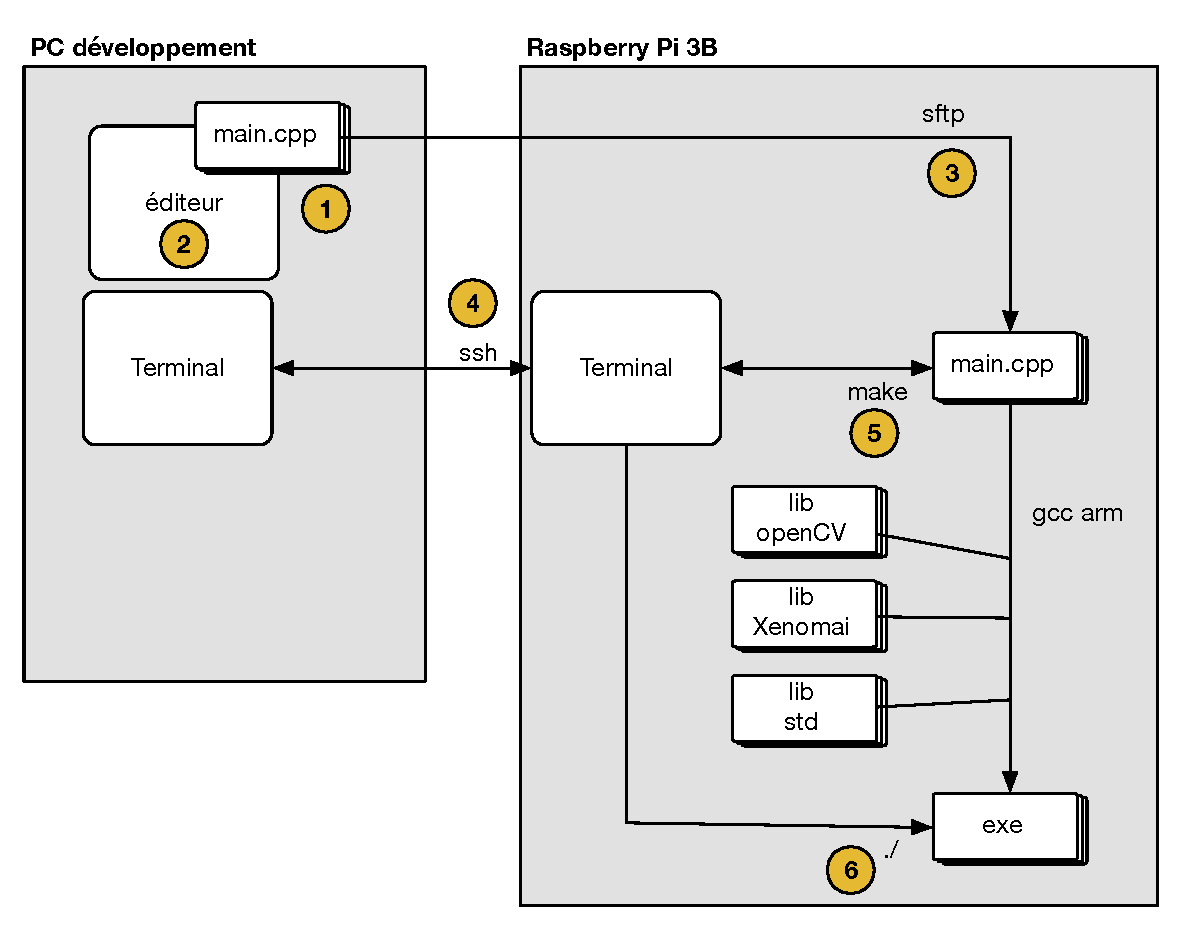
\includegraphics[scale=0.5]{./figures-pdf/edition2}
\caption{Edition locale et compilation distante}
\label{fig:edition2}
\end{center}
\end{figure}

Les étapes à suivre sont alors :
\begin{enumerate}
\item récupérer le code du dépôt (voir section~\ref{sec:git}) sur le PC,
 \item éditer le code avec l'outil que vous préférez,
 \item copier le code du PC vers la \raspi en utilisant la commande {\tt sftp} (voir ci-dessous),
\item se connecter de manière distante à la \raspi via ssh (voir section~\ref{sec:ssh}),
 \item compiler avec la commande {\tt make} à l'aide du {\tt Makefile} (qu'il faudra aussi avoir copié sur la \raspi),
 \item lancer l'exécutable par la commande {\tt sudo ./superviseur} (voir section ~\ref{sec:utilisation}).
 \end{enumerate}


\paragraph{Copie distante de fichiers :}
Il est possible d'utiliser {\tt sftp} pour copier un fichier d'une machine sur une autre. Pour cela, en se plaçant dans le répertoire où se trouve le fichier à copier, il faut exécuter les commandes suivantes :
\\ \indent\indent{\tt sftp pi@10.105.1.x} avec {\tt x} le numéro de la \raspi (mot de passe {\tt insa}),
\\ \indent\indent{\tt sftp > put file} avec {\tt file} le nom du fichier à copier,
\\ \indent\indent{\tt sftp > bye} pour quitter sftp.


%%%%%%%%%%%%%%%%%%%%
\subsection{Développement d'une application distante : édition locale et compilation distante (version Netbeans)}
%%%%%%%%%%%%%%%%%%%%

Cette deuxième solution applique le même schéma que précédemment (édition locale du code et compilation distante) mais en utilisant Netbeans comme IDE (figure~\ref{fig:edition2b}).

\begin{figure}[htbp]
\begin{center}
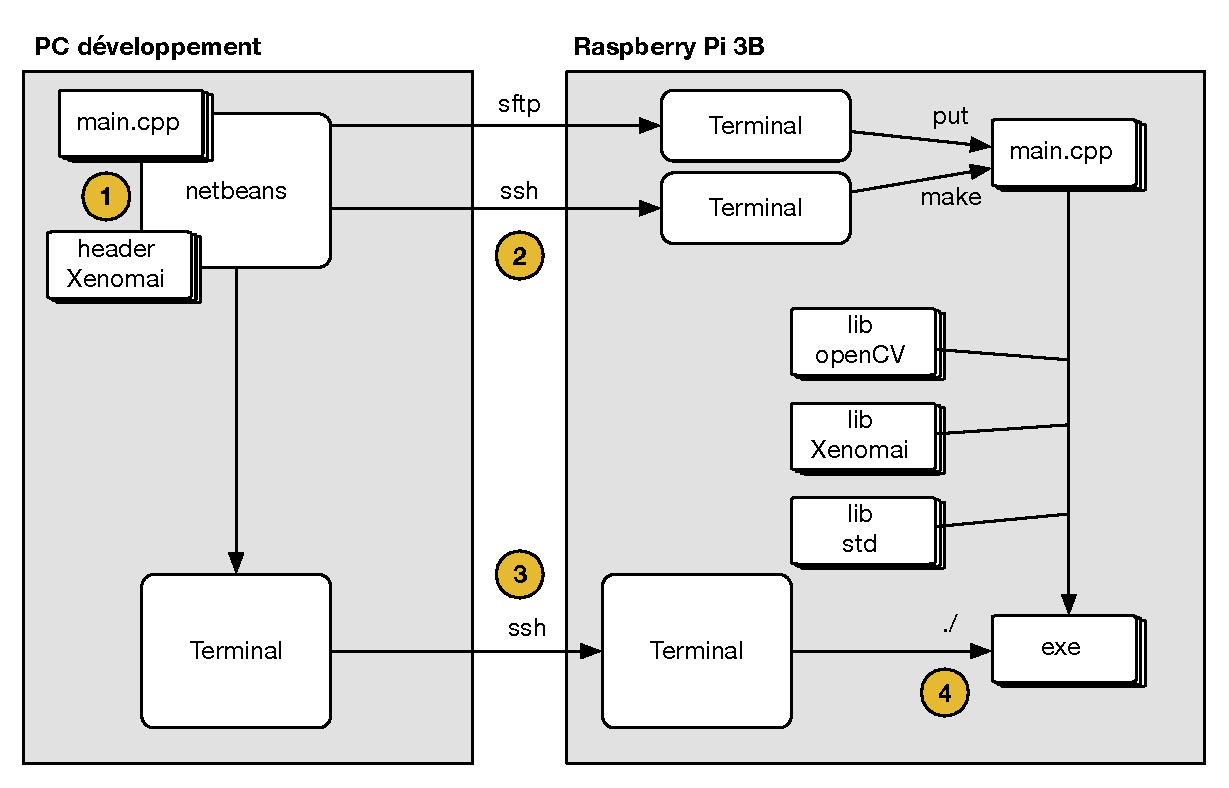
\includegraphics[scale=0.5]{./figures-pdf/edition2b}
\caption{Edition locale et compilation distante avec Netbeans}
\label{fig:edition2b}
\end{center}
\end{figure}

Cette solution peut sembler longue, mais une fois la configuration réalisée il en restera plus qu'à lancer les éléments automatiquement.

Les principales étapes sont :
\begin{enumerate}
\item éditer le code sur Netbeans,
\item lancer la compilation distante depuis Netbeans qui se chargera de copier les fichiers distants et de les compiler,
\item lancer un terminal depuis Netbeans,
\item exécuter le programme.
\end{enumerate}

\subsubsection{Récupérer le code}

Copiez localement (sur le PC) le dépôt git (voir section~\ref{sec:git}).

\todo[inline]{Mettre à jour en fonction du dépot}

\framebox[\textwidth]{
\begin{minipage}{0.9\textwidth}
Le projet initial est livré avec un projet Netbeans déjà configuré. Vous pouvez simplement l'ouvrir depuis... Il vous faudra ensuite simplement reconfigurer la cible en suivant les étapes présentées dans la section~\ref{sec:cible}.
\end{minipage}
}


\subsubsection{Créer un projet Netbeans}

\begin{enumerate}
\item Lancez Netbeans,
\item Allez dans {\tt File->new project},
\item Choisir {\tt C/C++} pour {\tt categories}, puis {\tt C/C++ Application},
\item Cliquez Next
\item Donner un nom au projet (ce sera par défaut le nom de votre exécutable),
\item Décocher {\tt Create main file},
\item cliquez sur  {\tt Finish},
\end{enumerate}

\subsubsection{Importer le code dans le projet}

\begin{enumerate}
\item Cliquez droit sur votre projet et choisissez {\tt Add existing items from Folders...},
\item puis {\tt Add Folder... } et allez chercher les répertoires que vous avez importé depuis github :
\begin{itemize}
\item {\tt superviseur\_robot/destijl\_init},
\item {\tt superviseur\_robot/src},
\end{itemize}
\item Cliquez {\tt Add}.
\end{enumerate}

Vous pouvez supprimer tous les autres répertoires du projet (clique droit sur les répertoires).

\subsubsection{Configurer une compilation distante}
\label{sec:cible}

\begin{enumerate}
\item Cliquez droit sur le projet et choisir {\tt Properties},
\item Allez dans l'onglet {\tt Build},
\item Choisir {\tt ...} pour {\tt Build Host},
\item Cliquez sur {\tt Add},
\item Remplir {\tt Hostname} avec {\tt 10.105.1.x} l'adresse de la \raspi,
\item Cliquez {\tt Next},
\item Saisir {\tt pi} pour le {\tt login},
\item Cliquez {\tt Next},
\item Attendre l'ouverture de la communication,
\item Saisir {\tt insa} comme mot de passe,
\item Sélectionner {\tt  SFTP} pour {\tt Access project files via},
\item Cliquez {\tt Finish},
\item Cliquez {\tt OK},
\item Cliquez {\tt Apply},
\item Cliquez {\tt OK}.
\end{enumerate}

\subsubsection{Configurer la compilation}

\begin{enumerate}
\item Cliquez droit sur le projet et choisir {\tt Properties},
\item Allez dans l'onglet {\tt Build->C++ Compiler},
\item Choisir {\tt ...} pour {\tt Additional Options},
\item Copier dans le champ {\tt -D\_GNU\_SOURCE -D\_REENTRANT -fasynchronous-unwind-tables -D\_\_MERCURY\_\_ -I/usr/xenomai/include/alchemy -g -D\_WITH\_TRACE\_ 

-I/usr/xenomai/include/ -I/usr/xenomai/include/mercury -MMD -MP} 
\item Cliquez {\tt OK},
\item Allez dans l'onglet {\tt Build->Linker},
\item Choisir {\tt ...} pour {\tt Additional Options},
\item Copier dans le champ {\tt  -D\_GNU\_SOURCE -D\_REENTRANT -fasynchronous-unwind-tables -D\_\_MERCURY\_\_ -I/usr/xenomai/include/alchemy -L/usr/xenomai/lib -lalchemy 

-lcopperplate -lmercury -L/opt/vc/lib -I/usr/local/include -lopencv\_highgui -lopencv\_core -lopencv\_imgproc -Wl,{-}{-}no-as-needed -lalchemy -lcopperplate 

/usr/xenomai/lib/xenomai/bootstrap.o -Wl,{-}{-}wrap=main 

-Wl,{-}{-}dynamic-list=/usr/xenomai/lib/dynlist.ld -L/usr/xenomai/lib -lmercury 

-lpthread -lrt -Wl,-rpath /usr/xenomai/lib -lopencv\_highgui -lopencv\_core 

-lopencv\_imgcodecs -lraspicam\_cv -lopencv\_imgproc -lpthread} 
\item Cliquez {\tt OK},
\item Cliquez {\tt Apply},
\item Cliquez {\tt OK}.
\end{enumerate}

\subsubsection{Tester la compilation}

\begin{enumerate}
\item Cliquez sur l'icone \og Marteau \fg ou allez dans {\tt Run->Build Project}.
\end{enumerate}

\subsubsection{Configurer l'exécution}

\begin{enumerate}
\item Cliquez droit sur le projet et choisir {\tt Properties},
\item Allez dans l'onglet {\tt Run},
\item Remplir le champ {\tt Run Command} avec {\tt sudo "\$\{OUTPUT\_PATH\}"},
\item Remplir le champ {\tt Console Type} avec {\tt Standard Output}.
\end{enumerate}

\subsubsection{Exécuter l'application (directement depuis Netbeans)}
\begin{enumerate}
\item Cliquez sur l'icone \og Play \fg ou allez dans {\tt Run->Build Project}.
\end{enumerate}

\subsubsection{Exécuter l'application (avec un terminal)}
\begin{enumerate}
\item Cliquez sur l'icone \og Terminal \fg dans la fenêtre de le console (ou lancer un terminal),
\item Connectez via ssh à la \raspi,
\item allez dans {\tt .netbeans/.../dist/...} avec la commande {\tt cd} pour trouver le résultat de la compilation,
\item lancez l'exécution via {\tt sudo ./app} avec {\tt app} le nom de votre application.
\end{enumerate}

\subsubsection{Ajouter les header dans le projet Netbeans}

\begin{enumerate}
\item Téléchargez les entêtes des services Xenomai depuis \href{https://moodle.insa-toulouse.fr/mod/resource/view.php?id=37439}{moodle},
\item Décompresser l'archive,
\item Cliquez droit sur le projet et choisir {\tt Properties},
\item Allez dans l'onglet {\tt Build->C++ Compiler},
\item Choisir {\tt ...} pour {\tt Include Headers},
\item Cliquez sur {\tt Add},
\item Sélectionner tous les fichiers {\tt .h} de l'archive chargée ({\tt ./include\_xenomai/include}),
\item Cliquez {\tt OK},
\item Cliquez {\tt Apply},
\item Cliquez {\tt OK}.
\end{enumerate}

Le service {\tt rt\_task\_create} n'est pas reconnu suite à cette manipulation car il est déclaré à travers une macro qui masque à Netbeans son existence. Le service restera donc souligné en rouge.

%%%%%%%%%%%%%%%%%%%%
\subsection{Développement d'une application distante : édition et compilation distantes}
%%%%%%%%%%%%%%%%%%%%

Cette dernière solution est à éviter. Elle consiste à éditer le code directement sur la \raspi et d'y lancer la compilation via un terminal (figure~\ref{fig:edition1}).

\begin{figure}[htbp]
\begin{center}
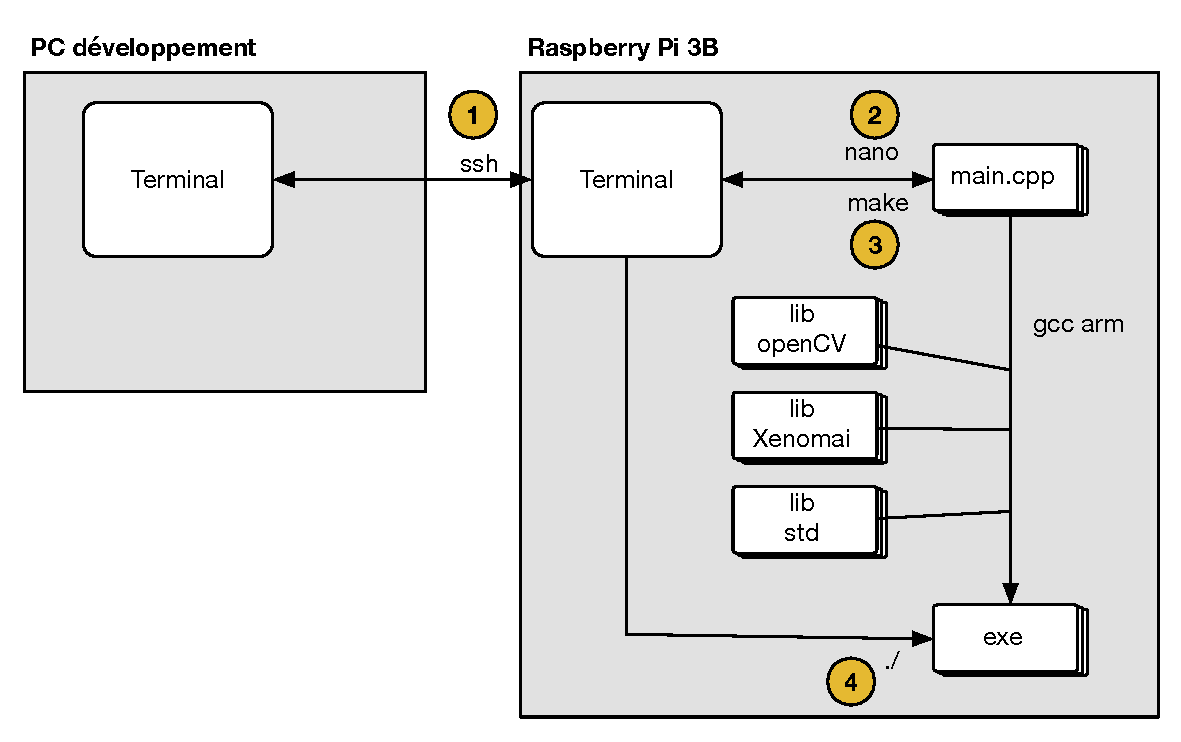
\includegraphics[scale=0.45]{./figures-pdf/edition1}
\caption{Edition et compilation distante}
\label{fig:edition1}
\end{center}
\end{figure}

Les étapes à suivre sont alors :
\begin{enumerate}
\item se connecter de manière distante à la \raspi via ssh (voir section~\ref{sec:ssh}),
 \item éditer à distance (par ex. avec {\tt nano}) le code,
 \item compiler avec la commande {\tt make} à l'aide du {\tt Makefile} du répertoire {\tt /destijl\_init},
 \item lancer l'exécutable par la commande {\tt sudo ./superviseur} (voir section ~\ref{sec:utilisation})\\
\end{enumerate}

Vous pouvez ensuite lancer le moniteur (voir section~\ref{sec:utilisation}) pour interragir avec l'application.

\end{document}